\documentclass[tikz,border=6pt]{standalone}
\usepackage{tikz}
\usetikzlibrary{arrows.meta,positioning,fit}
\definecolor{ink}{HTML}{222222}
\definecolor{inputfill}{HTML}{E8F1FF}
\definecolor{policyfill}{HTML}{FFF4D6}
\definecolor{outfill}{HTML}{EAF7EF}
\tikzset{
  box/.style={draw=ink, rounded corners=2pt, very thick, align=center, minimum height=8mm, text width=30mm, font=\sffamily\small},
  small/.style={draw=ink, rounded corners=2pt, thick, align=center, minimum height=7mm, text width=25mm, font=\sffamily\footnotesize},
  arrow/.style={-{Latex[length=2.2mm]}, very thick, draw=ink}
}
\begin{document}
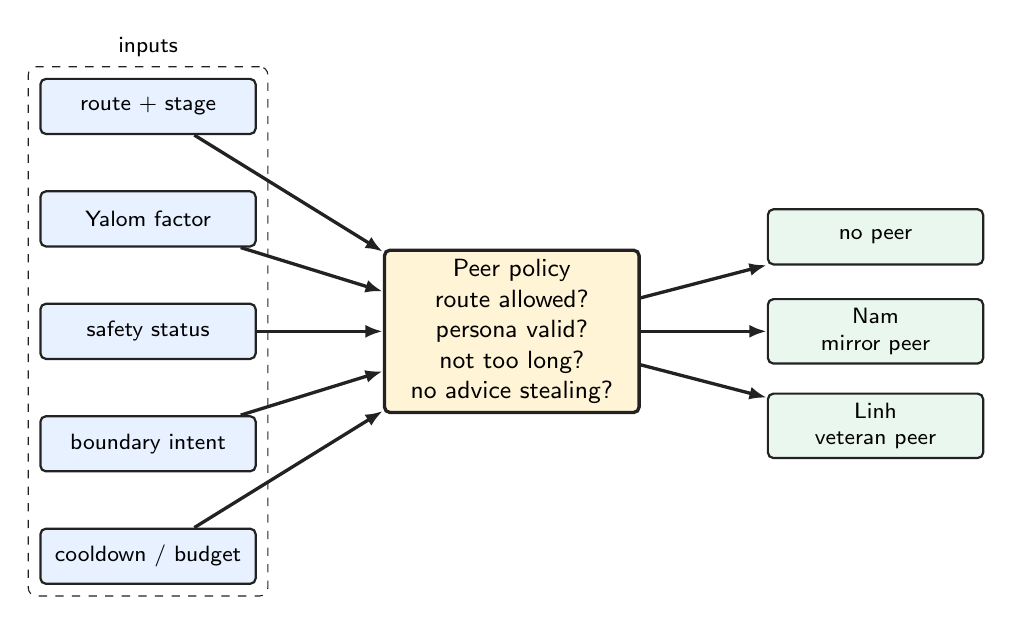
\begin{tikzpicture}[node distance=7mm and 8mm]
  \node[small, fill=inputfill] (route) {route + stage};
  \node[small, fill=inputfill, below=of route] (yalom) {Yalom factor};
  \node[small, fill=inputfill, below=of yalom] (safety) {safety status};
  \node[small, fill=inputfill, below=of safety] (boundary) {boundary intent};
  \node[small, fill=inputfill, below=of boundary] (cooldown) {cooldown / budget};

  \node[box, fill=policyfill, right=16mm of safety] (policy) {Peer policy\\route allowed?\\persona valid?\\not too long?\\no advice stealing?};

  \node[small, fill=outfill, right=16mm of policy, yshift=12mm] (none) {no peer};
  \node[small, fill=outfill, right=16mm of policy] (nam) {Nam\\mirror peer};
  \node[small, fill=outfill, right=16mm of policy, yshift=-12mm] (linh) {Linh\\veteran peer};

  \draw[arrow] (route) -- (policy);
  \draw[arrow] (yalom) -- (policy);
  \draw[arrow] (safety) -- (policy);
  \draw[arrow] (boundary) -- (policy);
  \draw[arrow] (cooldown) -- (policy);
  \draw[arrow] (policy) -- (none);
  \draw[arrow] (policy) -- (nam);
  \draw[arrow] (policy) -- (linh);

  \node[draw=ink, rounded corners=3pt, dashed, fit=(route)(yalom)(safety)(boundary)(cooldown), inner sep=4pt, label={[font=\sffamily\footnotesize]above:inputs}] {};
\end{tikzpicture}
\end{document}
